\documentclass[review]{elsarticle}

\usepackage[utf8]{inputenc}
\usepackage[T1]{fontenc}
\usepackage{graphicx}
\usepackage{amsmath}
\usepackage{amsfonts}
\usepackage{amssymb}
\usepackage{booktabs}
\usepackage{array}
\usepackage{multirow}
\usepackage{float}
\usepackage{url}
\usepackage{hyperref}

\journal{Radiation Physics and Chemistry}

\begin{document}

\begin{frontmatter}

\title{
    In Situ Spectral Analysis for Soil Carbon Measurement
    }

\author[uta]{Jose A. Cortes}
\ead{jose.cortes@uta.edu}

\author[uta]{Andrzej Korzeniowski}
\ead{korzeniowski@uta.edu}

\author[usda]{Galina Yakubova}
\ead{galina.yakubova@usda.gov}

\author[usda]{Aleksandr Kavetskiy}
\ead{aleksandr.kavetskiy@usda.gov}

\author[usda]{H. Allen Torbert}
\ead{allen.torbert@usda.gov}

\affiliation[uta]{organization={University of Texas at Arlington},
                 city={Arlington},
                 postcode={76019},
                 state={TX},
                 country={USA}}

\affiliation[usda]{organization={USDA ARS Auburn Lab},
                  city={Auburn},
                  state={AL},
                  country={USA}}

\begin{abstract}
Soil carbon is a key component of soil health and plays a crucial role in the global carbon cycle. 
Accurate measurement of carbon is essential for measuring soil quality and its impact on the environment. 
Traditional methods for measuring carbon are often time-consuming, expensive, and require laboratory analysis. 
In situ Neutron-Gamma spectral analysis (NGSA) offers an alternative for rapid and non-destructive measurement of soil carbon. 
This paper explores the use of NGSA techniques to measure carbon levels in various soil types. 
We simulate in MCNP6.2 common soil types and apply different NGSA methods, including peak fitting, component fitting, singular value decomposition, and deep learning, to evaluate their effectiveness in measuring of soil carbon. 
The results demonstrate that peak fitting with exponential falloff baseline achieves the lowest mean squared error ($7.66\times10^{-5}$), followed by component analysis methods. 
The study shows that NGSA methods can provide accurate soil carbon measurements, with convolution techniques improving overall accuracy across all methods.
\end{abstract}

\begin{keyword}
soil carbon \sep spectral analysis 
\sep gamma-ray spectroscopy \sep MCNP simulation 
\sep peak fitting \sep component analysis \sep deep learning
\end{keyword}

\end{frontmatter}

\section{Introduction}

Soil carbon is a key component of soil health and plays a crucial role in the global carbon cycle. Accurate measurement of carbon is essential for measuring soil quality, and its impact on the environment \cite{lal_soil_2018} Traditional methods for measuring carbon are often time-consuming, expensive, and require laboratory analysis \cite{de_ros_advancing_2025}. In situ spectral analysis offers an alternative for rapid and non-destructive measurement of soil carbon \cite{yakubova_tagged_2019}.  
This paper explores the use of NGSA techniques to measure carbon levels in various soil types. We simulate in MCNP6.2 common soil types and apply different NGSA methods, including peak fitting, component fitting, singular value decomposition, and deep learning, to evaluate their effectiveness in measuring soil carbon.

\section{Data Generation}

\subsection{Common Soil Types}

To investigate the effectiveness of NGSA methods for soil carbon measurement, we simulate a range of common soil types. The simulated data includes spectral readings across different wavelengths, capturing the unique spectral signatures of each soil type. This data serves as a foundation for applying various NGSA techniques.

\begin{table}[H]
\centering
\caption{Material compositions for soil simulation}
\label{tab:materials}
\begin{tabular}{lrrrrrrr}
\hline
 Material   &   C \% &   H \% &   O \% &   Si \% &   Na \% &   Al \% &   K \% \\
\hline
 Carbon     & 100.0 &   0.0 &   0.0 &    0.0 &    0.0 &    0.0 &   0.0 \\
 Water      &   0.0 &  11.2 &  88.8 &    0.0 &    0.0 &    0.0 &   0.0 \\
 Quartz     &   0.0 &   0.0 &  53.3 &   46.7 &    0.0 &    0.0 &   0.0 \\
 Feldspar   &   0.0 &   0.0 &  48.8 &   32.1 &    8.8 &   10.3 &   0.0 \\
 Mica       &   0.0 &   0.5 &  48.2 &   21.2 &    0.0 &   20.3 &   9.8 \\
\hline
\end{tabular}
\end{table}

Table \ref{tab:materials} presents the elemental composition of common soil materials used in the simulations. Mechanical mixing is used to combine materials based on their weight proportions, such that a 50\% carbon and 50\% water mix would have a composition of 50\% carbon, 5.6\% hydrogen, and 44.4\% oxygen. To measure the effectiveness of NGSA methods for carbon measurement, we simulate combinations of soil materials with varying carbon (C) and moisture (Water) content.

\subsection{Simulation in MCNP}

MCNP6 \cite{werner_mcnp_2017} was used to simulate gamma-ray spectra resulting from neutron activation of soil samples. Each simulation modeled a soil sample undergoing neutron activation with varying concentrations of carbon and other common soil constituents. The geometry was set up to mimic in situ measurement conditions, with a neutron source placed above a soil slab and a detector positioned to capture emitted gamma rays \cite{kavetskiy_neutron-stimulated_2017}.


In figure \ref{fig:mcnp_geometry}, the side view of the MCNP simulation setup is shown, highlighting the arrangement of the neutron source, soil slab, and detector. The geometry is designed to accurately represent the in situ conditions under which the soil samples are analyzed.

% \begin{figure}[H]
% \centering
% 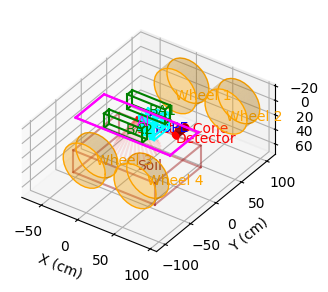
\includegraphics[width=0.8\textwidth]{../Figures/DataGeneration/MCNPGeometry.png}
% \caption{Geometry of MCNP simulation setup showing neutron source, soil slab, and detector configuration (Side View)}
% \label{fig:mcnp_geometry}
% \end{figure}

\begin{figure}[H]
\centering
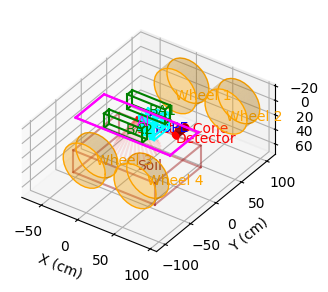
\includegraphics[width=0.8\textwidth,clip,trim=0cm 5cm 0cm 2cm]{../Figures/DataGeneration/MCNPGeometry.png}
\caption{Geometry of MCNP simulation setup showing neutron source, soil slab, and detector configuration (Side View)}
\label{fig:mcnp_geometry}
\end{figure}

In figure \ref{fig:mcnp_geometry_top}, the top view of the MCNP simulation setup is presented, providing a clear view of the spatial arrangement of the components, including the shielding around the detector to minimize background radiation.


\begin{figure}[H]
\centering
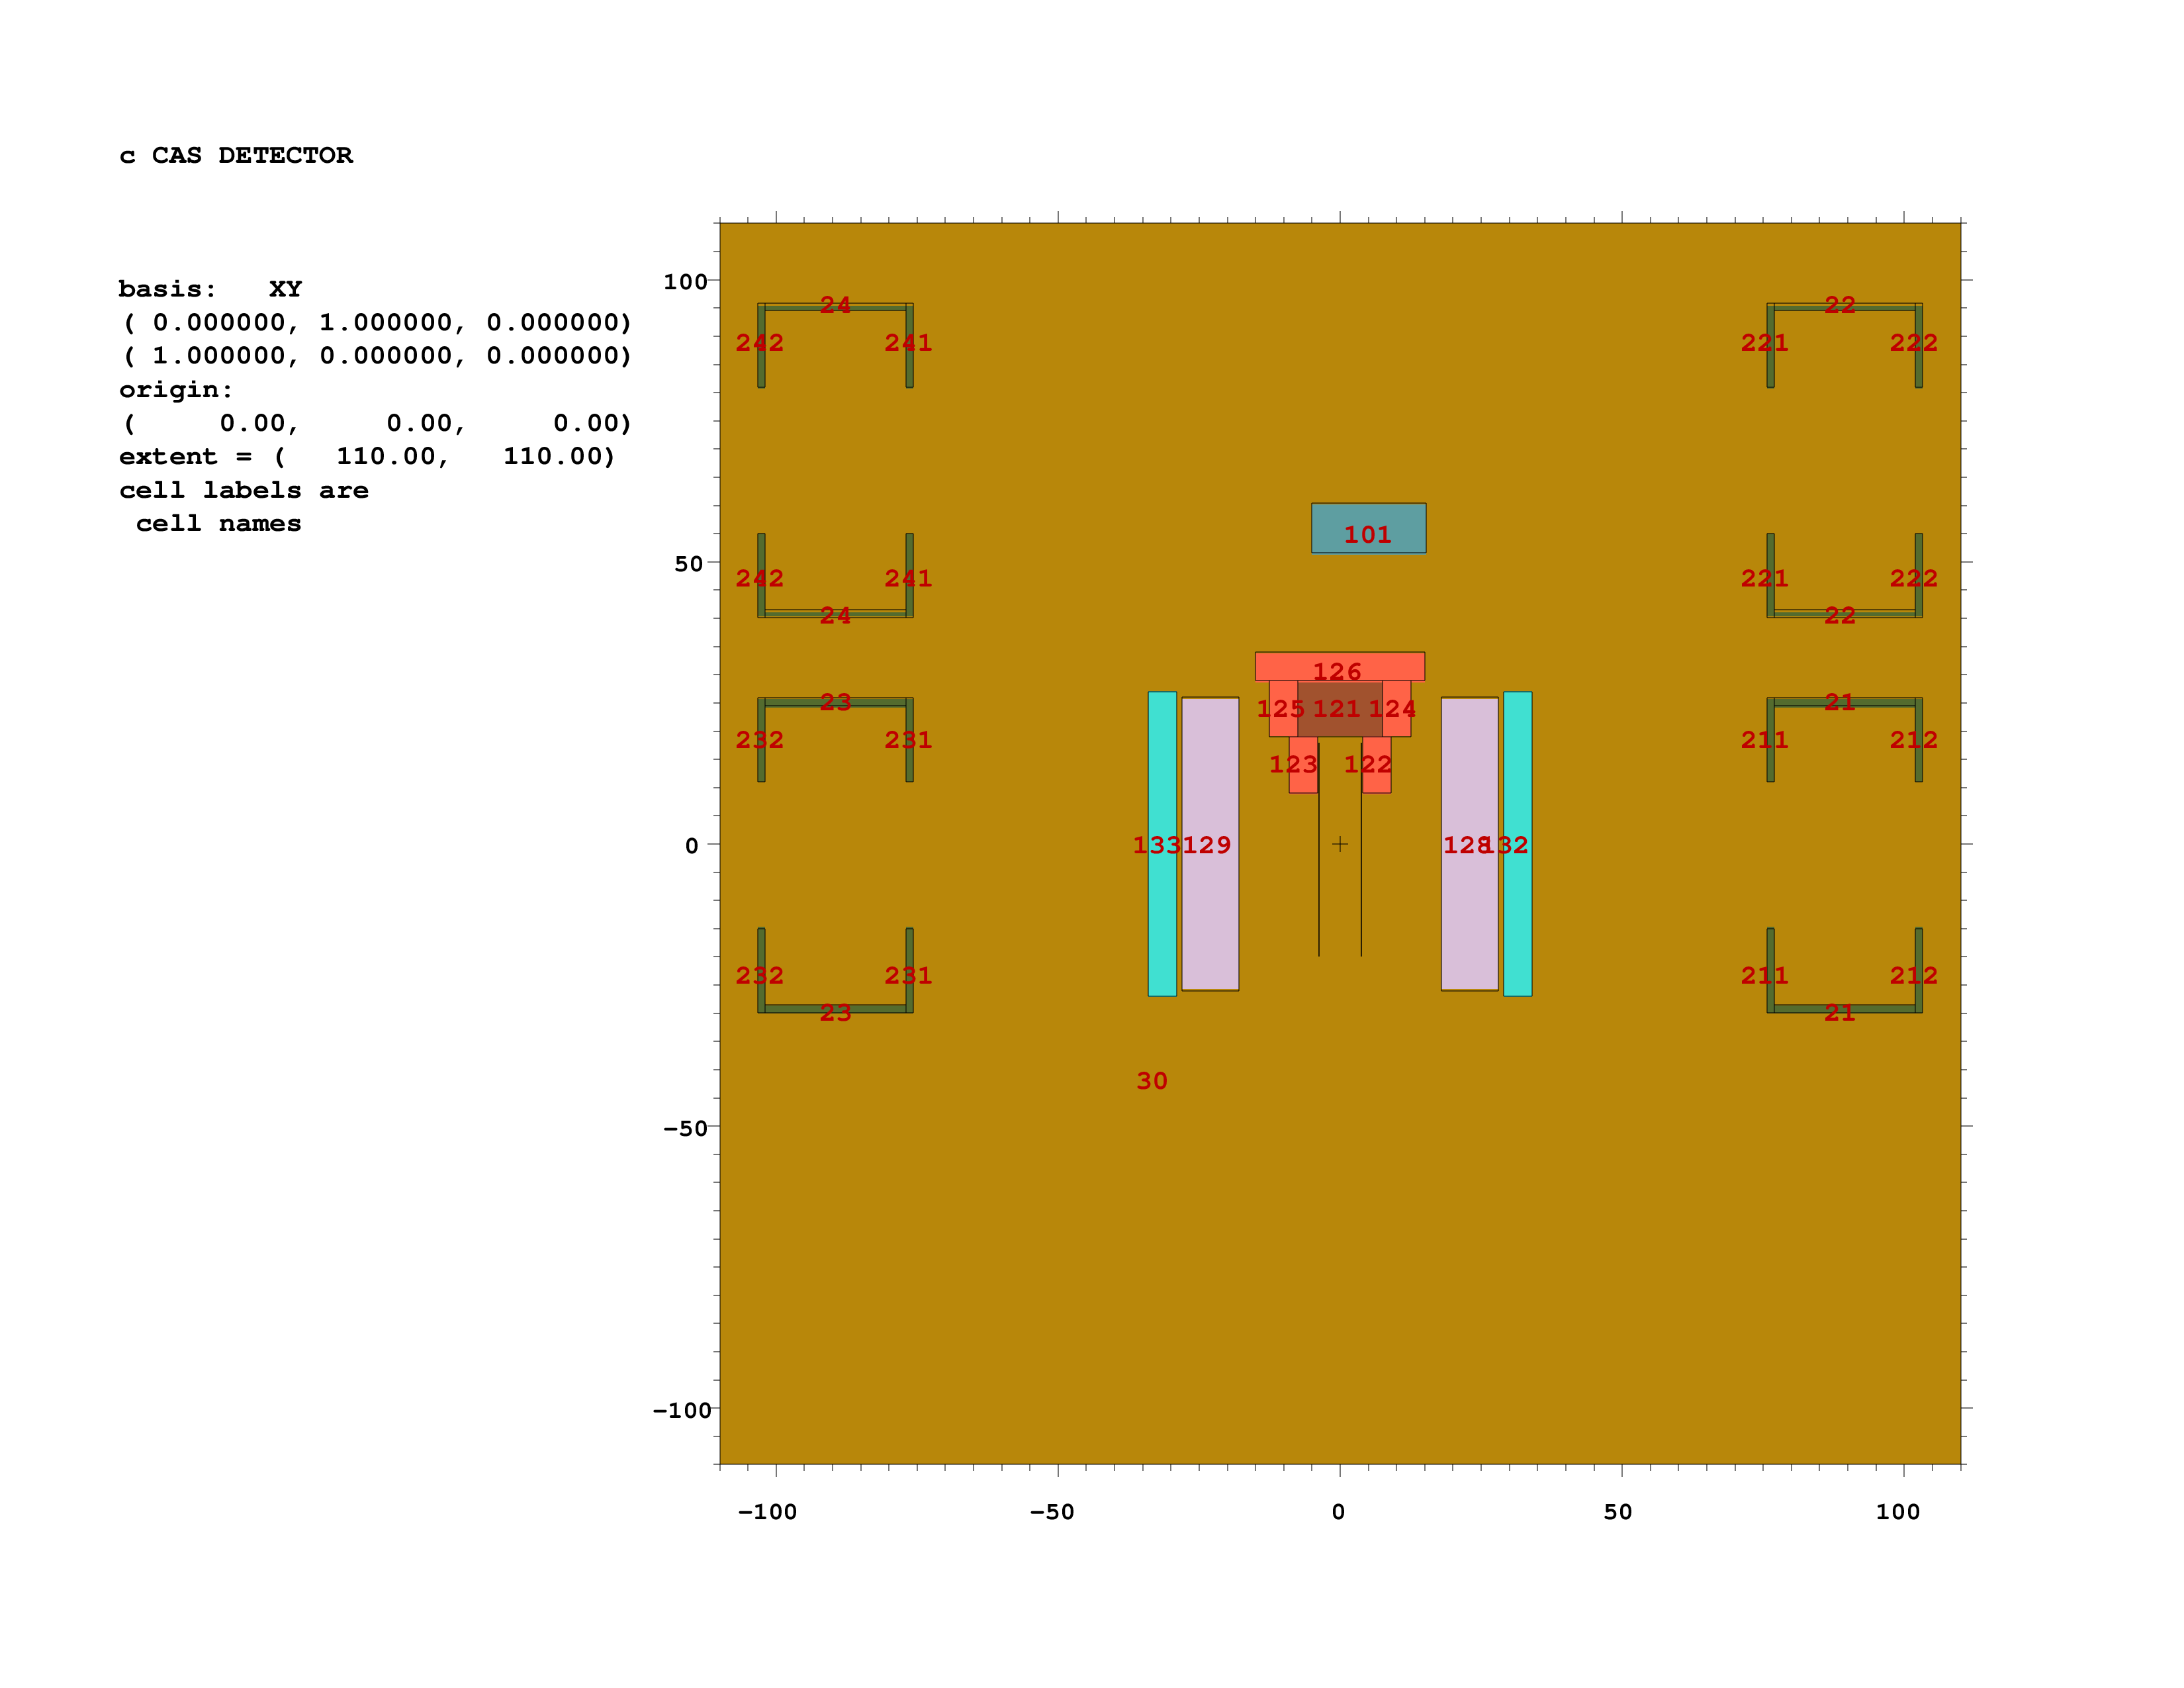
\includegraphics[width=0.8\textwidth]{../Figures/DataGeneration/top.png}
\caption{Cross section of MCNP simulation setup showing wheels and shielding (Top View)}
\label{fig:mcnp_geometry_top}
\end{figure}

Key simulation parameters included:
\begin{itemize}
\item \textbf{Neutron source energy:} API120 portable neutron (D-T generator) generator \cite{kavetskiy_energy_2018}
\item \textbf{Soil slab dimensions:} 112 cm × 90 cm × 30 cm
\item \textbf{Detector type:} NaI detector \cite{yakubova_measuring_2025}
\item \textbf{Tally:} F8 (pulse height tally) for gamma spectra
\end{itemize}

This approach enables the generation of realistic spectral data for a variety of soil compositions, forming the basis for evaluating different NGSA techniques. Table \ref{tab:chemical_identifiers} lists the MCNP chemical identifiers for the elements considered in the simulations.

\begin{table}[H]
    \centering
    \caption{MCNP Chemical Identifiers}
    \label{tab:chemical_identifiers}
    \begin{tabular}{lrrrrrrr}
    \hline
    Element         &    C &    H &    O &    Si &    Na &    Al &     K \\
    \hline
    MCNP Identifier & 6000 & 1001 & 8016 & 14000 & 11023 & 13027 & 19000 \\
    \hline
    \end{tabular}
\end{table}

\subsection{Spectral Readings}

The spectral readings obtained from the MCNP simulations provide a detailed distribution of the gamma-ray emissions from the soil samples per neutron, similar to what would be measured in a real-world scenario.

\begin{figure}[H]
\centering
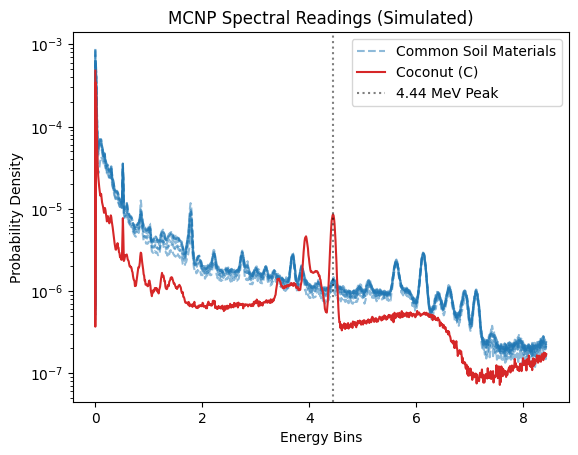
\includegraphics[width=0.8\textwidth]{../Figures/DataGeneration/MCNPSpectralReading.png}
\caption{Example MCNP spectral reading showing gamma-ray energy distribution}
\label{fig:mcnp_spectral}
\end{figure}

\subsection{Training and Testing Data}

The training data for the NGSA methods is picked from the edge cases of the simulated data. This includes the highest and lowest carbon levels both as would be found in simulation as well as natural soils. The testing data is all cases of the simulated data, excluding the training data. The data also ranges from 0\% to 80\% moisture content.

\begin{table}[H]
\centering
\caption{Carbon level classifications}
\label{tab:carbon_levels}
\begin{tabular}{ll}
\toprule
Carbon Level & Associated Amount \\
\midrule
Natural & 0\%-15\% Carbon \\
High & 15\%-80\% Carbon \\
\bottomrule
\end{tabular}
\end{table}

\begin{figure}[H]
\centering
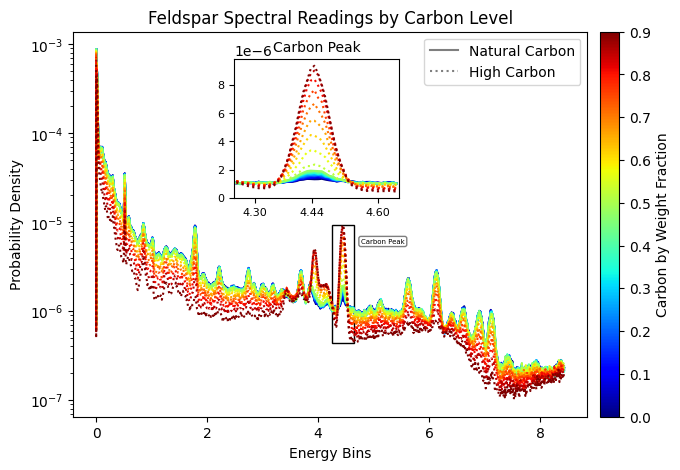
\includegraphics[width=0.8\textwidth]{../Figures/DataGeneration/FeldsparSpectralReadingByCarbonLevel.png}
\caption{Feldspar spectral reading by carbon level showing the variation in spectral signatures with different carbon concentrations}
\label{fig:feldspar_carbon}
\end{figure}

\subsection{Data Convolution}

In the context of NGSA, MCNP can be used to simulate the interaction of radiation with soil materials, providing spectrums to analyze. Linear Convolution is used to quickly predict spectral readings for material mixtures by combining the spectral signatures of individual components. This does not account for the complex interactions between materials, but it provides a simplified approach to generate spectral data for analysis. The error metric for this convolution method is based on the difference between the simulated spectral readings and the readings obtained from MCNP simulations. The effects of convolution as training data on the analysis results will be investigated in the results section.

\begin{figure}[H]
\centering
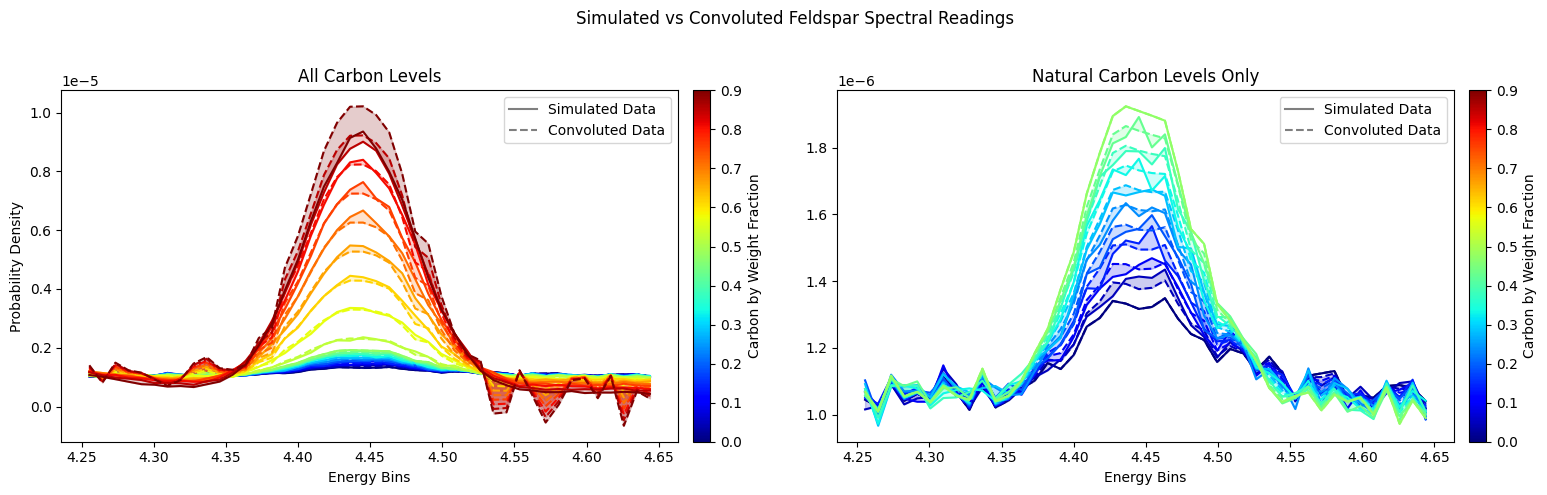
\includegraphics[width=0.8\textwidth]{../Figures/DataGeneration/Sim_vs_Convoluted_FeldsparSpectralReadings_Combined.png}
\caption{Comparison of simulated vs convoluted data for Feldspar spectral readings}
\label{fig:sim_vs_conv}
\end{figure}

\section{Analysis Methods of Spectral Readings}

This section explores various spectral analysis methods applied to the simulated spectral readings. Each method is evaluated for its effectiveness in measuring Carbon levels. Error is calculated using mean squared error (MSE) between the predicted and actual carbon levels in the test data.

\subsection{Calibration Layer}

All models undergo a calibration process to align their predictions with the carbon measurements. This involves a regression model between a key characteristic and the predicted values. A linear regression model is used for this purpose.

The Scipy python package is used for the fitting process\cite{virtanen_scipy_2020}, leveraging its curve fitting capabilities to refine the initial parameter estimates. All fitting problems are taken as fitting a curve f(x, p0) where p0 are the initial parameters. The fitting process iteratively adjusts these parameters to minimize the difference between the predicted and actual values, using a least-squares approach. The Levenberg-Marquardt algorithm is employed to optimize the fitting process\cite{more_levenberg-marquardt_1978}. When the fitting is bounded, Trust Region Reflective optimization \cite{branch_subspace_1999} is used.

\subsection{Peak Baseline Fitting}

Peak fitting involves using the least-squares method in identifying and quantifying the baseline and peaks in the spectral data that correspond to specific soil components \cite{gardner_use_2011}. This method is useful for extracting information about the concentration of individual elements or compounds in the soil. For effective peak fitting, the data is filtered to focus on the peak area.

The fitting function is defined as:
\begin{equation}
F_f = F_p + F_b
\end{equation}

where $F_p$ is the peak function (e.g., Gaussian) and $F_b$ is the baseline function (e.g., linear or exponential falloff).

\begin{table}[H]
\centering
\caption{Function parameterizations for peak fitting}
\label{tab:functions}
\begin{tabular}{ll}
\toprule
Function Type & Example Expression \\
\midrule
Linear & $ax + b$ \\
Exp Falloff & $a \cdot \exp(-b \cdot x) + c$ \\
Gaussian & $a \cdot \exp(-((x - b)^2)/c^2) + d$ \\
\bottomrule
\end{tabular}
\end{table}

The baseline function is subtracted from the fitted function to isolate the peak, and the area under the peak is calculated to quantify the concentration of the corresponding element or compound in the soil.

\begin{figure}[H]
\centering
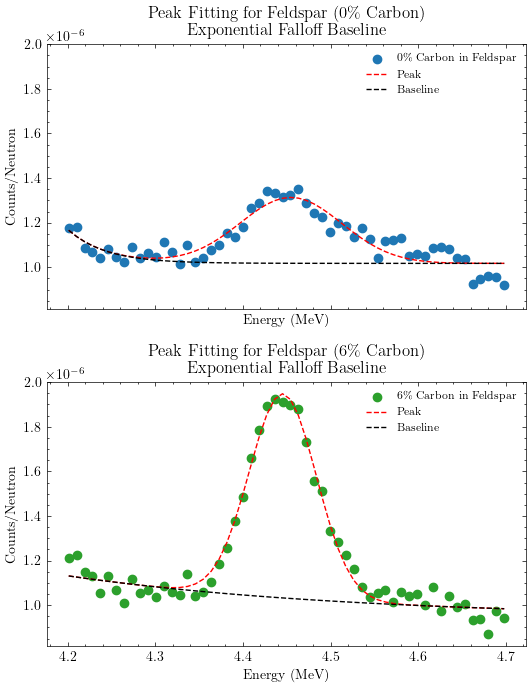
\includegraphics[width=0.8\textwidth]{../Figures/Analysis/peak_fitting_feldspar_subplots.png}
\caption{Peak fitting example showing fitted peak and baseline for feldspar spectrum}
\label{fig:peak_fitting}
\end{figure}

The final prediction is calibrated using the peak areas.

\begin{figure}[H]
\centering
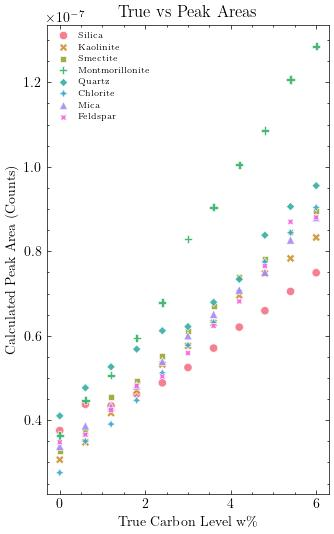
\includegraphics[width=0.8\textwidth]{../Figures/Analysis/carbon_level_vs_predicted_pf.jpg}
\caption{Peak fitting prediction results showing carbon level vs predicted values}
\label{fig:peak_predictions}
\end{figure}

\subsection{Component Fitting}

Component fitting involves modeling the spectral data as a combination of known spectral signatures of soil components. This method allows for the estimation of the concentration of multiple components in the soil based on their spectral contributions.

The combined spectral function is defined as:
\begin{equation}
F_c = \sum_{i} A_i \cdot F_i
\end{equation}

where $F_c$ is the combined spectral function, $A_i$ are the coefficients representing the concentration of each component, and $F_i$ are the spectral functions of individual components.

% \begin{figure}[H]
% \centering
% 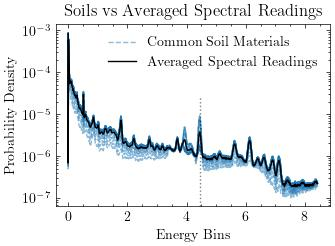
\includegraphics[width=0.8\textwidth]{../Figures/DataGeneration/CommonSoilSpectravsAverageSoilSpectrum.jpg}
% \caption{Common soil spectra vs average soil spectrum showing the spectral signatures of different soil components}
% \label{fig:common_soil_spectra}
% \end{figure}

\begin{figure}[H]
\centering
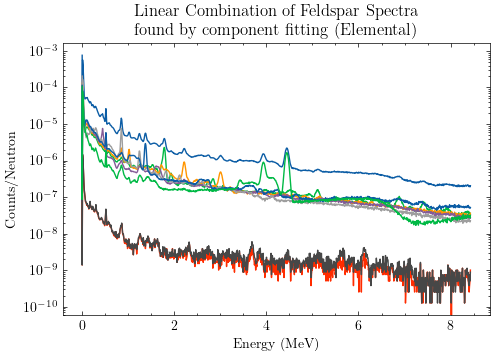
\includegraphics[width=0.8\textwidth]{../Figures/Analysis/elemental_linear_combination_feldspar.png}
\caption{Component fitting process showing linear combination of elemental spectral components for feldspar analysis}
\label{fig:elemental_component_fitting}
\end{figure}

\begin{figure}[H]
\centering
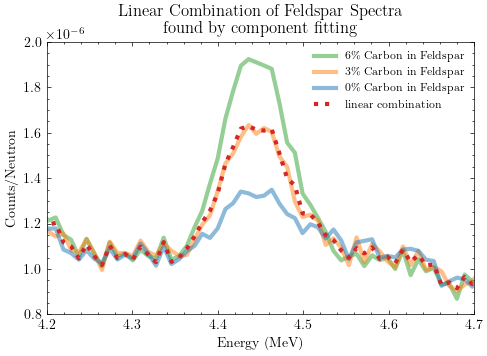
\includegraphics[width=0.8\textwidth]{../Figures/Analysis/linear_combination_feldspar.png}
\caption{Component fitting process showing linear combination of spectral components for feldspar analysis}
\label{fig:component_fitting}
\end{figure}

Components can be any known spectral signature, either from pure elemental samples \cite{kavetskiy_neutron_2023} as shown in figure \ref{fig:elemental_component_fitting} or derived from soil samples similar to the target soil \ref{fig:component_fitting}. The fitting process involves adjusting the coefficients $A_i$ to minimize the difference between the combined spectral function $F_c$ and the observed spectral data. This method also benefits from filtering of low energy signals which are generally more likely to be caused by noise.

The carbon coefficient $A_C$ is then used to estimate the Carbon level in the soil. This method is particularly useful for analyzing complex soil mixtures where multiple known components contribute to the spectral signature. This method is also generalizable to study other elements or compounds.

\begin{figure}[H]
\centering
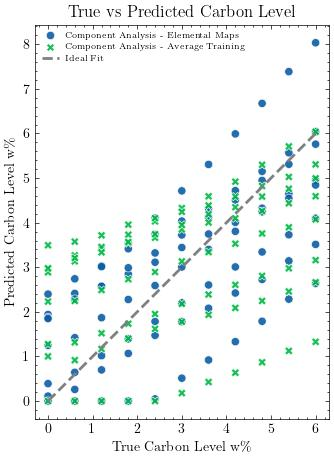
\includegraphics[width=0.8\textwidth]{../Figures/Analysis/carbon_level_vs_predicted_component_analysis.jpg}
\caption{Component fitting prediction results showing carbon level vs predicted values}
\label{fig:component_predictions}
\end{figure}

\subsection{Convex Optimization}

Convex optimization techniques can be applied to the spectral data to identify and quantify the contributions of different soil components. By formulating the problem as a convex optimization task, it is possible to find the optimal coefficients for the spectral components that minimize the difference between the observed and modeled spectra.

\begin{figure}[H]
\centering
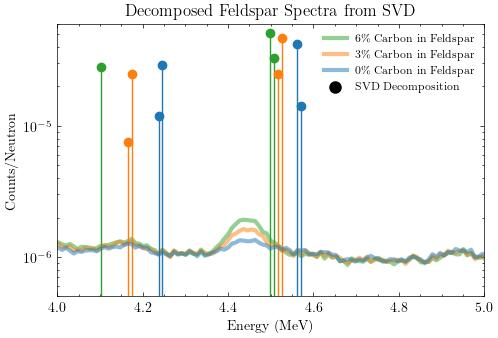
\includegraphics[width=0.8\textwidth]{../Figures/Analysis/decomposed_feldspar_svd.jpg}
\caption{Convex optimization process showing SVD decomposition of feldspar spectral data}
\label{fig:svd_decomposition}
\end{figure}

\begin{figure}[H]
\centering
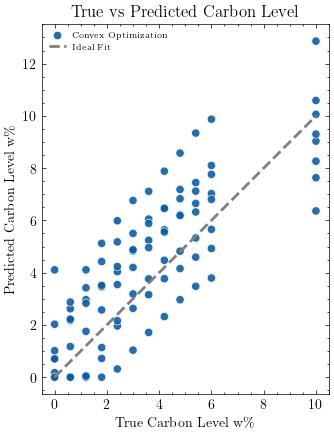
\includegraphics[width=0.8\textwidth]{../Figures/Analysis/carbon_level_vs_predicted_convex_optimization.jpg}
\caption{Convex optimization predictions showing carbon level vs predicted values using SVD}
\label{fig:svd_predictions}
\end{figure}

\subsection{Deep Learning}

Deep learning techniques, such as convolutional neural networks (CNNs), can be applied to spectral data for feature extraction and classification. These methods can learn complex relationships in the data and provide robust predictions of carbon levels based on spectral readings. The most important difference between deep learning and the previous methods is that it requires a large amount of training data to be effective. One method by Kim et al. \cite{kim_deep_2025} uses a deep learning model to predict existence, concentration and carbon peak areas.

\begin{figure}[H]
\centering
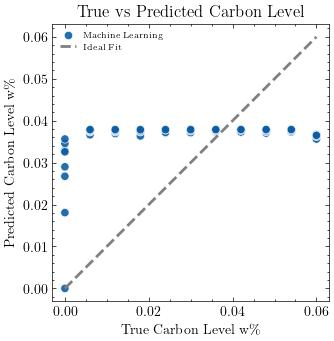
\includegraphics[width=0.8\textwidth]{../Figures/Analysis/carbon_level_vs_predicted_ml_optimization.jpg}
\caption{Deep learning prediction results showing carbon level vs predicted values using machine learning optimization}
\label{fig:ml_predictions}
\end{figure}


\section{Results}

The effectiveness of each method in measuring carbon levels is evaluated based on accuracy using mean squared error (MSE) as the metric. The results are summarized in Table~\ref{tab:results}.

\begin{table}[H]
\centering
\caption{Performance comparison of spectral analysis methods}
\label{tab:results}
\begin{tabular}{llc}
\toprule
Method Group & Method & MSE \\
\midrule
Peak Fitting & Exponential Falloff Baseline & $7.66 \times 10^{-5}$ \\
Component Analysis & Elemental Maps & $2.10 \times 10^{-4}$ \\
Component Analysis & Average Training & $3.43 \times 10^{-4}$ \\
Peak Fitting & Linear Baseline & $3.52 \times 10^{-4}$ \\
Machine Learning & Deep Learning & $3.67 \times 10^{-4}$ \\
Convex Optimization & SVD & $4.27 \times 10^{-4}$ \\
\bottomrule
\end{tabular}
\end{table}

\subsection{Comparing Analysis Methods}

Peak fitting with exponential falloff baseline is the most effective method for measuring carbon levels in soil, achieving the lowest MSE ($7.66 \times 10^{-5}$). Component analysis methods also perform well, with elemental maps achieving the second-best performance. The deep learning method shows promise but requires further optimization to improve its performance.

\subsection{Effects of Carbon Levels on Results}

\begin{table}[H]
\centering
\caption{Method performance by carbon level}
\label{tab:carbon_level_effects}
\begin{tabular}{lccccccc}
\toprule
Carbon Level & \multicolumn{7}{c}{MSE Values} \\
\cmidrule(lr){2-8}
& Peak Fitting & Peak Fitting & Component & Component & Convex & Filtered ML & Machine \\
& (Exp Falloff) & (Linear) & (Average) & (Elemental) & Optimization & & Learning \\
\midrule
Agricultural & $7.66 \times 10^{-5}$ & $3.52 \times 10^{-4}$ & $3.43 \times 10^{-4}$ & $2.10 \times 10^{-4}$ & $4.27 \times 10^{-4}$ & $3.70 \times 10^{-3}$ & $3.67 \times 10^{-4}$ \\
All & $1.42 \times 10^{-2}$ & $3.48 \times 10^{-2}$ & $1.92 \times 10^{-2}$ & $1.92 \times 10^{-2}$ & $2.64 \times 10^{-2}$ & $1.33 \times 10^{-1}$ & $1.01 \times 10^{-1}$ \\
\bottomrule
\end{tabular}
\end{table}

Lower carbon levels tend to result in higher MSE values across all methods, indicating that the spectral signatures of low-carbon soils are less distinct and more challenging to analyze accurately. The methods generally perform better with higher carbon concentrations, where the spectral features are more pronounced.

\subsection{Effects of Convolution on Results}

\begin{table}[H]
\centering
\caption{Method performance by training dataset type}
\label{tab:convolution_effects}
\begin{tabular}{lccccccc}
\toprule
Dataset & \multicolumn{7}{c}{MSE Values} \\
\cmidrule(lr){2-8}
& Peak Fitting & Peak Fitting & Component & Component & Convex & Filtered ML & Machine \\
& (Exp Falloff) & (Linear) & (Average) & (Elemental) & Optimization & & Learning \\
\midrule
Convolution Training & $7.26 \times 10^{-5}$ & $3.50 \times 10^{-4}$ & $2.95 \times 10^{-4}$ & $1.91 \times 10^{-4}$ & $2.93 \times 10^{-4}$ & $3.65 \times 10^{-4}$ & $3.61 \times 10^{-4}$ \\
Feldspar & $3.43 \times 10^{-5}$ & $3.60 \times 10^{-4}$ & $7.48 \times 10^{-7}$ & $7.92 \times 10^{-7}$ & $2.14 \times 10^{-3}$ & $1.10 \times 10^{-2}$ & $9.30 \times 10^{-4}$ \\
Material Mixes & $7.66 \times 10^{-5}$ & $3.52 \times 10^{-4}$ & $3.43 \times 10^{-4}$ & $2.10 \times 10^{-4}$ & $4.27 \times 10^{-4}$ & $3.70 \times 10^{-3}$ & $3.67 \times 10^{-4}$ \\
\bottomrule
\end{tabular}
\end{table}

Convolution generally improves the accuracy of spectral analysis methods by smoothing out noise and enhancing the signal-to-noise ratio. The results show that convolution leads to lower MSE values across all methods, indicating that it is beneficial for spectral analysis in soil carbon measurement.

\section{Discussion}

\subsection{Conclusions}

The study demonstrates the potential of spectral analysis methods for measuring soil carbon levels. Peak fitting and component fitting methods show the best performance, while deep learning techniques require further refinement. Convolution is beneficial for improving the accuracy of spectral analysis.

The peak fitting method with exponential falloff baseline achieved the highest accuracy, suggesting that proper baseline correction is crucial for effective spectral analysis. Component analysis methods provide a good balance between accuracy and interpretability, making them suitable for practical applications.

\subsection{Future Work}

Future work will focus on:
\begin{itemize}
\item Optimization of deep learning architectures for spectral analysis
\item Investigation of hybrid methods combining multiple analysis techniques
\item Field validation of the proposed methods
\item Extension to other soil properties beyond carbon content
\end{itemize}

\section{Acknowledgments}

We acknowledge the contributions of the USDA scientists for their guidance and support in this research. The spectral data generated in this study is available for further research and validation.

\bibliographystyle{elsarticle-num}
\bibliography{references}

\end{document}